\documentclass[10pt]{article}

%Math
\usepackage{amsmath}
\usepackage{amsfonts}
\usepackage{amssymb}
\usepackage{amsthm}
\usepackage{ulem}
\usepackage{stmaryrd} %f\UTF{00FC}r Blitz!
\usepackage{multirow}
\usepackage{multicol}

%PageStyle
\usepackage[ngerman]{babel} % deutsche Silbentrennung
\usepackage[utf8]{inputenc} 
\usepackage{fancyhdr, graphicx}
\usepackage[scaled=0.92]{helvet}
\usepackage{enumitem}
\usepackage{parskip}
\usepackage[a4paper,top=2cm]{geometry}
\setlength{\textwidth}{17cm}
\setlength{\oddsidemargin}{-0.5cm}


% Shortcommands
\newcommand{\Bold}[1]{\textbf{#1}} %Boldface
\newcommand{\Kursiv}[1]{\textit{#1}} %Italic
\newcommand{\T}[1]{\text{#1}} %Textmode
\newcommand{\Nicht}[1]{\T{\sout{$ #1 $}}} %Streicht Shit durch

%Arrows
\newcommand{\lra}{\leftrightarrow} 
\newcommand{\ra}{\rightarrow}
\newcommand{\la}{\leftarrow}
\newcommand{\lral}{\longleftrightarrow}
\newcommand{\ral}{\longrightarrow}
\newcommand{\lal}{\longleftarrow}
\newcommand{\Lra}{\Leftrightarrow}
\newcommand{\Ra}{\Rightarrow}
\newcommand{\La}{\Leftarrow}
\newcommand{\Lral}{\Longleftrightarrow}
\newcommand{\Ral}{\Longrightarrow}
\newcommand{\Lal}{\Longleftarrow}

% Code listenings
\usepackage{color}
\usepackage{xcolor}
\usepackage{listings}
\usepackage{caption}
\DeclareCaptionFont{white}{\color{white}}
\DeclareCaptionFormat{listing}{\colorbox{gray}{\parbox{\textwidth}{#1#2#3}}}
\captionsetup[lstlisting]{format=listing,labelfont=white,textfont=white}
\lstdefinestyle{JavaStyle}{
 language=Java,
 basicstyle=\footnotesize\ttfamily, % Standardschrift
 numbers=left,               % Ort der Zeilennummern
 numberstyle=\tiny,          % Stil der Zeilennummern
 stepnumber=5,              % Abstand zwischen den Zeilennummern
 numbersep=5pt,              % Abstand der Nummern zum Text
 tabsize=2,                  % Groesse von Tabs
 extendedchars=true,         %
 breaklines=true,            % Zeilen werden Umgebrochen
 frame=b,         
 %commentstyle=\itshape\color{LightLime}, Was isch das? O_o
 %keywordstyle=\bfseries\color{DarkPurple}, und das O_o
 basicstyle=\footnotesize\ttfamily,
 stringstyle=\color[RGB]{42,0,255}\ttfamily, % Farbe der String
 keywordstyle=\color[RGB]{127,0,85}\ttfamily, % Farbe der Keywords
 commentstyle=\color[RGB]{63,127,95}\ttfamily, % Farbe des Kommentars
 showspaces=false,           % Leerzeichen anzeigen ?
 showtabs=false,             % Tabs anzeigen ?
 xleftmargin=17pt,
 framexleftmargin=17pt,
 framexrightmargin=5pt,
 framexbottommargin=4pt,
 showstringspaces=false      % Leerzeichen in Strings anzeigen ?        
}

%Config
\renewcommand{\headrulewidth}{0pt}
\setlength{\headheight}{15.2pt}

%Metadata
\fancyfoot[C]{If you use this documentation for an exam, you should offer a beer to the authors!}
\title{
	\vspace{2cm}
	\textbf{Software Construction}
}
\author{Florian Thiévent}
\date{3. Semester (HS 2018)}


% hier beginnt das Dokument
\begin{document}

% Titelbild
\maketitle
\begin{center}
\vspace{3cm}
	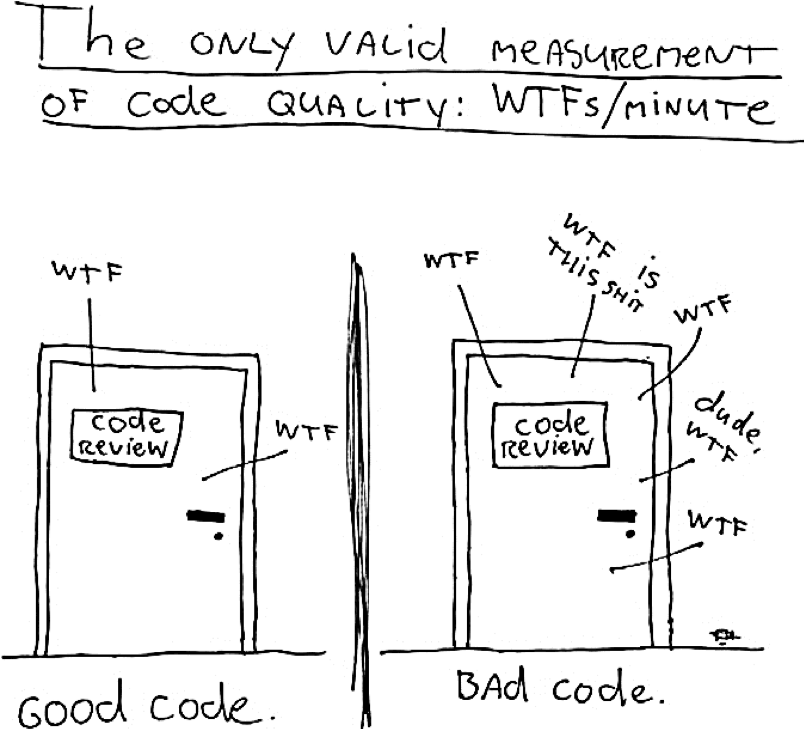
\includegraphics{assets/Titelbild.png}
\thispagestyle{fancy}
\end{center}

\newpage

% Inhaltsverzeichnis
\pagenumbering{Roman}
\tableofcontents	  	


\newpage
\setcounter{page}{1}
\pagenumbering{arabic}

% Inhalt Start

\section{Software Construction}
\begin{tabular}{p{50mm} p{50mm} p{50mm}}
	\begin{center}
		Problem Definition \newline
		Anforderungen spezifizieren\newline
		\textbf{Planung der Anwendung}\newline
		SoftwareArchitektur\newline
	\end{center}
	& 
	\begin{center}
		\textbf{\uline{Detail Plan}}\newline
		\textbf{\uline{Coding and Debugging}}\newline
		\textbf{\uline{Unit Testing}}\newline
	\end{center}
	& 
	\begin{center}
		Team Management\newline
		Maintenance (Betrieb)\newline
		\textbf{Integration}\newline
		\textbf{Integration Testing}\newline
		System Testing\newline
	\end{center}
\end{tabular}

\subsection{Definition}
Software construction is a fundamental act oft software engineering: the construction of working, \textbf{meaningful software} through a combination of \textbf{coding, validation and testing} by a programmer.
\subsection{Low Level SWC}
\begin{itemize}
	\item Testing definieren
	\item Design und Klassen schreiben
	\item Erstellen und Naming der Variablen und Konstanten
	\item Unit Testing, Integration Testing und Debugging
	\item Review von anderem Code von Teammitgliedern
	\item Integration von Software
	\item Formatierung von Code und Kommentaren
\end{itemize}

\subsection{Wieso ist SWC wichtig}
\textbf{Construction is the only activity that's guaranteed to be done}
\begin{center}
	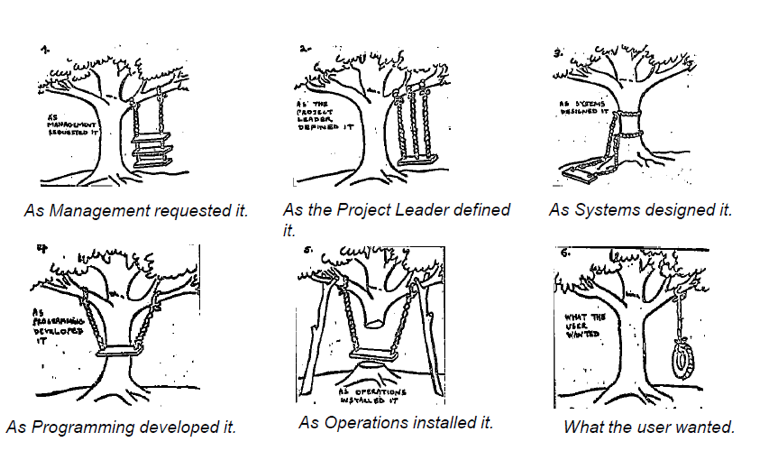
\includegraphics[width=0.8\textwidth]{assets/typical_project}
\end{center}

\subsection{Software Qualität}
\begin{itemize}
	\item Reliability: Zuverlässige Software welche fehlerfrei betrieben werden kann
	\item Reusability: Code Teile auch für andere Projekte nutzbar machen
	\item Extendibility: Erweiterbarkeit soll einfach möglich sein
	\item Understandability: Code soll verständlich für andere sein
	\item Efficiency: Geschwindigkeit
	\item Usability: Software einfach nutzen, auf das Zielpublikum ausgerichtet
	\item Portability: Einfach in eine andere Umgebung zügeln
	\item Functionality: Software soll funktional sein
\end{itemize}
\textbf{Definition ISO:} The totality of features and characteristics of a product or service that bear on its ability stated or implied needs
\\
\textbf{Definition IEEE:} The degree to which a system, component, or process meets specified requirements.

\subsection{Ziele}
Die Software muss den Anforderungen des Kunden entsprechen. \textbf{"Good enough Software" not excellent software!}

\subsection{Extreme Programming}
\begin{enumerate}
	\item Der Kunde/Auftraggeber ist immer verfügbar
	\item Code wird gemäss vereinbarten Standards programmiert
	\item Zuerst die Tests programmieren, dann den eigentlichen Code
	\item Der produktive Code wird immer zu zweit programmiert
	\item Nur ein Programmierer-Paar darf gleichzeitig Code integrieren
	\item Integriere häufig
	\item Jeder hat auf den gesamten Code Zugriff
	\item Optimiere so spät wie möglich
	\item Keine Überstunden
	\item Das Team folgt gemeinsamen Code-Richtlinien, so dass es aussieht, als wenn der Code von einer einzigen Person geschrieben worden wäre
	\item XP Projekte werden in sehr kurzen Abständen released (von täglich bis zu maximal alle 3-4 Wochen)
\end{enumerate}

\section{Version Control System}
Es geht grundsätzlich um sich ständig ändernde Artefakte welche verwaltet werden müssen. Jede Änderung soll eindeutig nachvollziehbar sein.

\subsection{Motivation für eine VCS}
Ohne Versionsmanagement sieht der Alltag von Entwicklern so aus:
\begin{itemize}
	\item Bugs die behoben wurden tauchen plötzlich wieder auf
	\item Dateien gehen verloren
	\item Frühere Releases der Software können nicht mehr erstellt werden
	\item Dateien werden "auf mysteriöse Art und Weise" verändert
	\item Gleicher oder ähnlicher Code existiert mehrfach in verschiedenen Projekten
	\item Zwei Entwickler ändern dieselbe Datei gleichzeitig ohne es zu merken
\end{itemize}

\subsection{Problem of Filesharing}
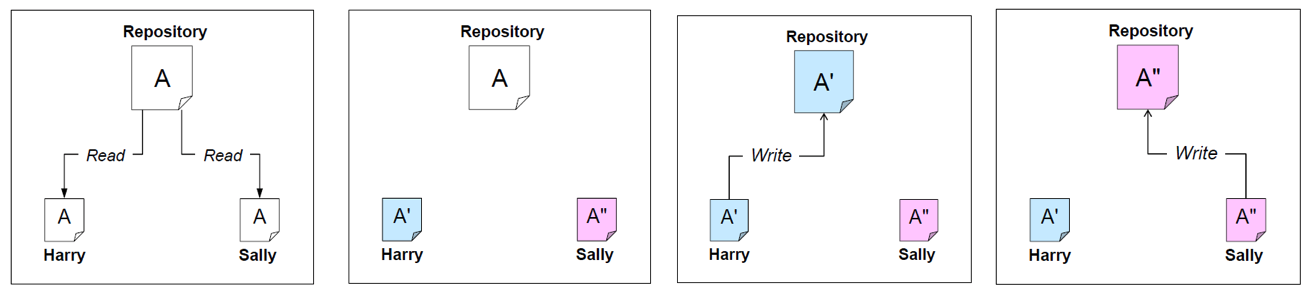
\includegraphics[width=0.9\textwidth]{assets/problem_of_filesharing.png}

\subsection{Lock-Modify-Unlock Solution}
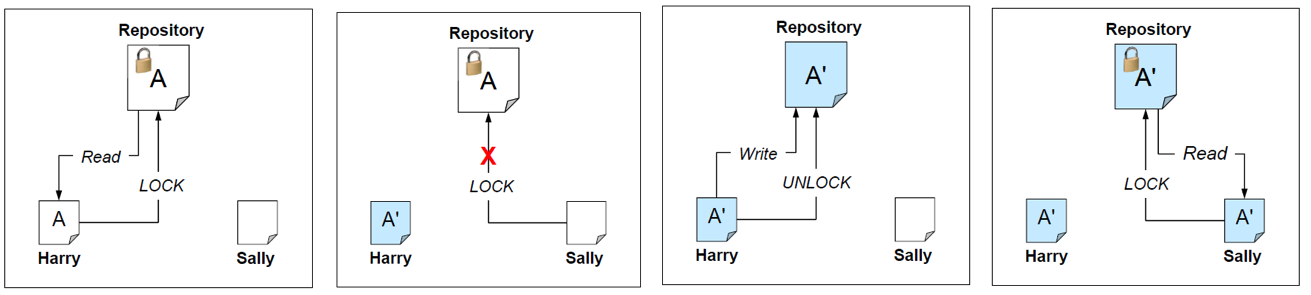
\includegraphics[width=0.9\textwidth]{assets/lock_modify_unlock_solution.png}

\subsection{Copy-Modify-Merge Solution}
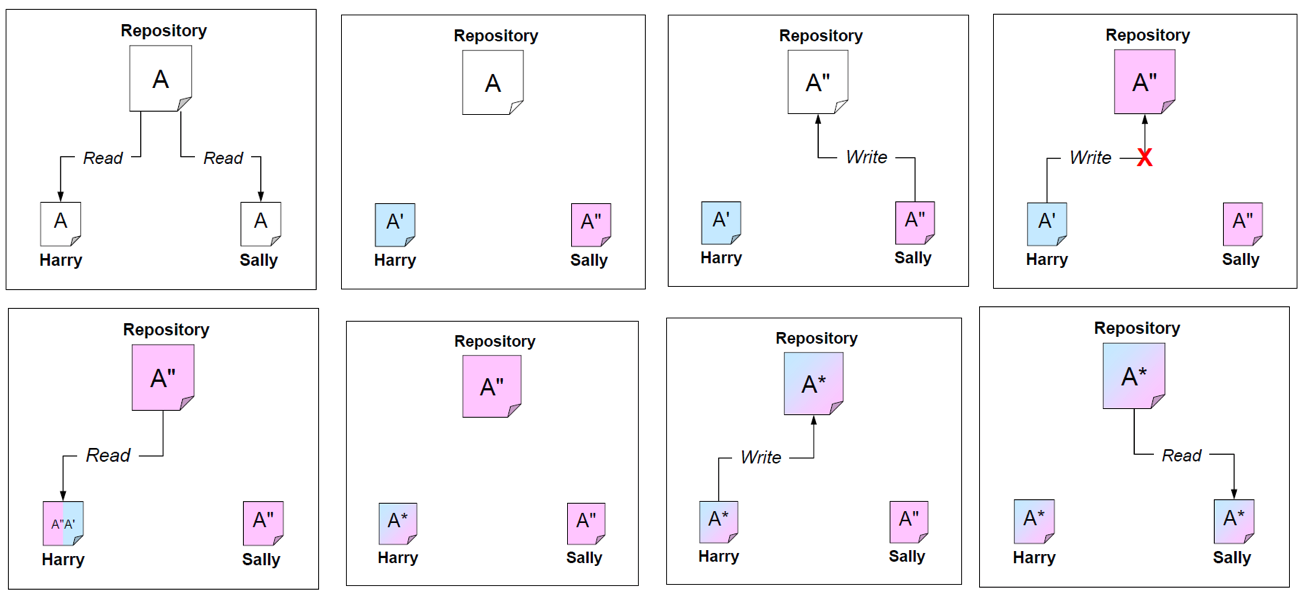
\includegraphics[width=0.9\textwidth]{assets/copy_modify_merge_solution.png}

\subsection{Grundbegriffe Versions- und Release-Management}
\subsubsection{Version}
Ein Zustand eines Konfigurationselementes mit einem klar definierten Funktionsumfang.
\subsubsection{Release}
Bezeichnet eine veröffentlichte Version eines Konfigurationselementes. Oft wird ein Release auch ausserhalb der Software-Entwicklungsorganisation zusammengestellt.
\subsubsection{Major}
Die Idee, das Major-Versionen (mindestens teilweise) inkompatibel sind
\subsubsection{Minor}
Änderungen dieser Nummer sind rückwärts kompatibel.
\subsubsection{Patch}
Bug-Fixes, Änderungen sind vorwärts- und rückwärts kompatibel.
\subsubsection{Build}
Diese Nummer gibt eine Neukompilierung von Sourcecode an, z.B. aufgrund von Prozessor-, Plattform- oder Compileränderungen.
\subsubsection{Revision}
Kleine Änderung an einer Version, welche Fehler behebt, jedoch keine Einfluss auf den Funktionsumfang haben.
\subsubsection{Variante}
Eine Variation einer Version welche entwickelt wurde um z.B. auf einer anderen Hardware oder unter einem anderen Betriebssystem zu laufen. Oder auch um für verschiedene Benutzergruppen feine Anpassungen vorzunehmen.  Beispiele: Anpassungen für Tablets, Sehbehinderte, Touchscreens.
\subsection{Grundbegriffe VCS}
\subsubsection{Repository}
Eine Datenbank in welcher Projektdateien gespeichert werden. Ein Repository vergisst nichts, d.h. es ist nicht möglich eine Datei zu überschreiben. Vielmehr wir einfach eine neue Version der Datei gespeichert, die alte bleibt weiterhin im Repository und es kann auch weiterhin zugegriffen werden.
\subsubsection{Working Copy}
Eine \textit{lokale Kopie} aller relevanten Projektdateien. Der Entwickler arbeitet immer auf dieser lokalen Kopie. Es wird also \textit{nie} direkt auf den Dateien im Repository gearbeitet.
\subsubsection{Checkout / Clone}
Ist die Bezeichnung für einen Vorgang wenn eine Working Copy vom Repository bezogen wird. Dies ist eine reine Leseoperation auf dem Repository. Dabei wird auf der Entwicklermaschine eine neue Working Copy angelegt.
\subsubsection{Commit / Push}
Bezeichnet den Vorgang wenn eine Datei oder ein ganzes Set an Dateien (neu oder geändert) \textit{mit einer Beschreibung} ins Repository gespeichert wird. Man spricht auch davon diese unter Versionskontrolle zu stellen. Dies ist eine Schreiboperation auf dem Repository die \textit{atomar} erfolgt, d.h. pro Commit werden entweder alle oder gar keine Dateien ins Repository gespeichert. Damit ist sichergestellt, das das Set an Dateien konsistent ins Repository gespeichert wird. Es ist nicht möglich, dass durch zwei gleichzeitige Commits die Dateien durcheinandergebracht werden.
\subsubsection{Update / Fetch / Pull}
Bezeichnet den Vorgang wenn Dateien aus dem Repository mit der eigenen Working Copy abgeglichen werden. Indem andere Entwickler ihre Arbeit committen erhält das Repository neue Versionen welche auf den Working Copies der anderen Entwickler noch nicht vorhanden sind. Der Abgleich findet auf der Working Copy statt, für das Repository ist ein Updatevorgang somit eine reine Leseoperation.
\subsubsection{Revision, Version}
Jeder Commit verändert den Inhalt des Repositories und erzeugt somit eine neue Version oder Revision des Repositories die eindeutig identifizierbar sein muss. Dies ist notwendig um später wieder auf einen bestimmten Stand der Arbeit zurückzukehren zu können. Manche Repositories verwenden mehrstellige Versionsnummern (z.B. CVS), andere nummerieren die Commits einfach durch (z.B. Subversion) oder vergeben einen Hash (z.B. Git) als Identifikation.
\subsubsection{Entwicklungsverlauf (Baseline, Codeline, Line of Development}
TODO
\subsubsection{Branch}
TODO
\subsubsection{Merging}
TODO
\subsubsection{Tag, Label}


\subsection{Configuration Items}
\begin{center}
\begin{tabular}{|lll|c} 
\hline
Unter VCS & Nicht im VCS & Grenzfall \\
\hline
Sourcen & Testprotokolle (generiert) & DB \\
Dokumentation & Testreports (generiert) & Video \\ 
Kommunikation & Persönliche Konfig (IDE) & Audio \\
Tests & Javadoc $\rightarrow$ html &  \\
Geteilte Config & DIE & \\
Video / Audiofiles (kleine) & Compilate &\\
& (.exe, .class, .jar & \\
 & Files aus anderen Projekten & \\ 
 & (Libraries, Vorlagen) & \\

\hline
\end{tabular}
\end{center}

\section{Build - Automation}
Die Komponenten einer Software werden per Knopfdruck erstellt. Macht meist mehrer Dinge auf einmal (Code compilieren, Tests durchlaufen, Checkout, Kopie auf Server, E-Mail). Der Buildvorgang kann auch automatisch gestartet werden.
\subsection{Wieso wird dies benötigt, Probleme}
TODO
\subsection{Build Prozess}
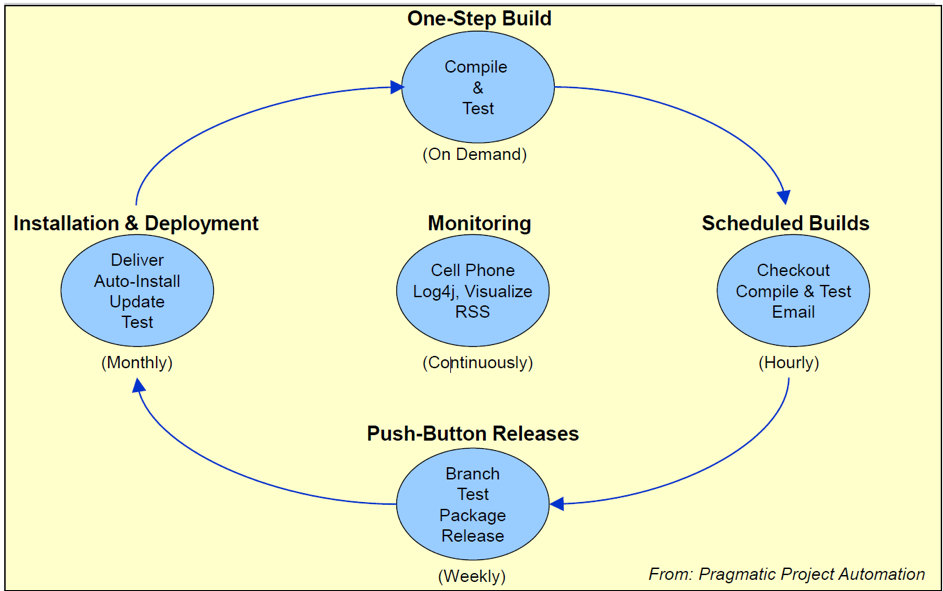
\includegraphics{assets/buildprozess.png}



% Inhalt Ende 
\end{document} 









